\chapter{Modèles stochastiques}

\section{Concepts de base}

Une expérience aléatoire est une expérience dont le résultat n'est pas connu avec certitude.
Supposons que tous les résultats possibles de cette expérience soient connus.
L'espace d'échantillonnage $\Omega$ est cet ensemble de résultats possibles d'une expérience aléatoire.

\begin{example}[Espace d'échantillonnage]
\mbox{}\\
 \begin{itemize}
  \item 
   Tirage d'une pièce de monnaie: $\Omega = \lbrace P,F \rbrace$.
  \item
  Lancement d'un dé: $\Omega  = \lbrace 1,2,3,4,5,6 $.
 \item
  Temps écoulé avant l'arrivée d'un premier client dans un magasin ouvert durant 8 heures, depuis sont ouverture: $\Omega =[0,8]$.
 \end{itemize}
\end{example}

Un événement $E$ est un sous-ensemble de l'espace échantillonnage.
Supposons que nous répétions l'expérience aléatoire un grand nombre de fois ($n$),
et que l'événement E se produise $m$ fois.
La probabilité associée à l'événement $E$ peut être approchée comme
\[
 P[E] \approx \frac{m}{n}. 
\]
Une définition empirique de la probabilité de $E$ est (en version fréquentiste)
\[
 P[E] = \lim_{n \rightarrow \infty} \frac{m}{n}, 
\]
De manière plus formelle
\begin{definition}
$P$ est une mesure de probabilité si
\begin{itemize}
 \item 
  $0 \leq P[E] \leq 1$, pour tout $E \subset \Omega$;
 \item
  $P[ \emptyset ] = 0$ et $P[ \Omega] = 1$;
 \item
  $P[E_1 \cup E_2] = P[E_1] + P[E_2]$, si $E_1$ et $E_2$ sont disjoints (i.e. $E_1 \cap E_2 = \emptyset$).
\end{itemize}
\end{definition}

\begin{example}
 Tirage d'une pièce de monnaie: $P[ \lbrace P \rbrace ] = P[ \lbrace F \rbrace ]= 0.5$.
\end{example}

L'occurence un événement $E_1$ se produit peut influencer la probabilité d'un autre événement $E_2$.
Par exemple, la probabilité qu'il pleuve demain ($E_2$) est plus élevée s'il pleut aujourd'hui ($E_1$) que s'il ne pleut pas.
Si $P[E_1] > 0$, nous définissons la probabilité conditionnelle associée à l'événement $E_2$, étant donné $E_1$, comme:
\[
P[E_2\,|\,E_1 ] = \frac{P[ E_1 \cap E_2 ]}{P[E_1]}.
\]
La probabilité conditionnelle jouit des propriétés suivantes:
\begin{itemize}
 \item 
  $0 \leq P[E_2\,|\,E_1] \leq 1$;
 \item
  $P[ \emptyset\,|\, E_1] = 0$ et $P[  \Omega\,|\,E_1\ ] = 1$;
 \item
  $P[E_2 U E_3\,|\,E_1) = P[E_2\,|\,E_1] + P[E_3\,|\,E_1]$, si $E_2$ et $E_3$ sont disjoints.
\end{itemize}

Deux événements $E_1$ et $E_2$ sont indépendants si
\[
 P[E_2\,|\,E_1] = P[E_2]. 
\]
De manière alternative, nous pouvons utiliser les définition suivantes:
\begin{align*}
P[E_1\,|\,E_2] &= P[E_1] \\
P[E_1 \cap E_2] &= P[E_1]P[E_2].
\end{align*}
En général, nous postulons l'indépendance de deux événements pour se servir des définitions ci-dessus,
plutôt que de déduire l'indépendance de deux événements à partir des définitions.
$K$ événements $E_1$, $E_2$,\ldots, $E_k$ sont indépendants si
\[
P[E_1 \cap E_2 \cap \ldots E_k] = P[E_1]P[E_2]\ldots P[E_k].
\]

\section{Variable aléatoire}

Une variable aléatoire $X$ est une fonction qui associe une valeur numérique
$X(s)$ à chaque élément $s$ de l'espace d'échantillonnage:
\[
X: \Omega \rightarrow \RR.
\]
Il existe deux types principaux de variables aléatoires:
\begin{itemize}
 \item 
 variable aléatoire continue: valeurs réelles;
 \item
 variable aléatoire discrète: valeurs entières ou nombre fini de valeurs.
\end{itemize}

\begin{example}[Lancer de dés]
Considérons l'expérience aléatoire du lancer de deux dés.
L'espace d'échantillonnage est $\Omega = \lbrace (1,1),(1,2),\ldots,(6,6) \rbrace$.
Une variable aléatoire $X$ serait la somme des résultats des deux dés. Ainsi, par exemple,
\begin{align*}
P[X=2] &= P[s \in \Omega\,:\, X(s)=2] = P[(1,1)] = \frac{1}{36}; \\
P[X \leq 4] &= P[s \in \Omega\,:\, X(s) \leq 4] =
P[(1,1),(1,2),(1,3),(2,1),(2,2),(3,1)] = \frac{6}{36} = \frac{1}{6}.
\end{align*}
\end{example}

La fonction de répartition associée à une variable aléatoire $X$ est définie comme
\[
 F_X(b) = P[X \leq b] = P[s \in \Omega \,|\, X(s) \leq b], 
\]
Elle a comme propriétés:
\begin{itemize}
 \item 
 non décroissante;
 \item
 $\lim_{b \rightarrow -\infty} F_X(b) = 0$ et $lim_{b\rightarrow \infty} F_X(b) = 1$;
 \item
 $P[a < X \leq b] = F_X(b) - F_X(a)$, vu que
 \[
 \lbrace s \in \Omega\,:\, X(s) \leq b \rbrace =
 \lbrace s \in \Omega\,:\,X(s)\leq a \rbrace \cup \lbrace s \in \Omega \,:\, a < X(s) \leq b \rbrace.
 \]
\end{itemize}

\begin{example}[Lancer de dés]
Soit $X$ la somme des résultats des deux dés. Nous avons
\begin{align*}
 F_X(1) &= P[X \leq 1] = 0;\\
 F_X(2) &= P[X \leq 2] = P[X=2] = \frac{1}{36};\\
 F_X(4) &= P[X \leq 4] = \frac{6}{36} = \frac{1}{6};\\
 F_X(12) &= P[X \leq 12] = 1.\\
\end{align*}
\end{example}

\subsection{Variables aléatoires discrètes}

La  fonction de masse associée à une variable aléatoire $X$ est définie comme
\[
P_X(k) = P[X=k] = P[s \in \Omega\,:\, X(s)=k ].
\]
Pour une variable aléatoire discrète, nous avons
\[
F_X(b) = P[X \leq b] = \sum_{k \leq b} P[X=k] = \sum_{X \leq b} P_X(k).
\]
aussi,
\[
P[a<X<b] = F_X(b) - F_X(a) - P_X(b).
\]
\begin{example}[Lancer de dés]
 Soit $X$ la somme des résultats des deux dés. Alors,
\begin{align*}
F_X(2) &= P[X \leq 2] = P[X=2] = P_X(2) = \frac{1}{36}; \\
F_X(4) &= P[X \leq 4] = P[X=2] + P[X=3] + P[X=4] = P_X(2) + P_X(3) + P_X(4) = \frac{6}{36} = \frac{1}{6}.
\end{align*}
\end{example}

\subsection{Variables aléatoires continues}

Une variable aléatoire X est continue si sa fonction de répartition peut être représentée ainsi:
\[
F_X(b) = \int_{-\infty}^b f_x(x) dx.
\]
La fonction sous l'intégrale est appelée fonction de densité et satisfait les conditions suivantes:
\begin{align*}
& f_x(x) \geq 0,\ \forall x; \\
& \int_{-\infty}^{\infty} f_x(x) dx = 1
\end{align*}
Si la fonction de densité est continue, alors elle est égale à la dérivée de la fonction de répartition:
\[
f_X(x) = \frac{dF_X}{dx}(x).
\]
La fonction de masse prend toujours la valeur 0:
\[
P_X(x) = 0,\ \forall x.
\]
Pour tout intervalle de la forme $<a,b>$, nous avons également
\[
P[X \in <a,b> ] = \int_a^b f (x)dx = F_X(b) - F_X(a).
\]

\subsection{Espérance mathématique}

L'espérance mathématique  (moyenne) associée à une variable aléatoire $X$ est dénotée $E[X]$ et définie comme suit:
\[
E[X] = \begin{cases}
\sum_k kP_X(k) = \sum_k P[X=k] & \mbox{si $X$ est discrète},\\
\int_{-\infty}^{\infty} x f_X(x) dx & \mbox{si $X$ est continue}.
\end{cases}
\]

\begin{example}[Lancer de deux dés]
Soit $X$ la somme des résultats des deux dés.
\[
E[X] = \sum_k P[X=k] = \sum_{k=2^12} kP[X=k] = 7.
\]
\end{example}

Nous pouvons également considérer l'espérance d'une fonction $g(X)$.
Si $X$ est une variable aléatoire discrète, cela donne
\[
E[g(X)] = \sum_k g(k) P_X(k).
\]
Pour une variable continue, nous aurons
\[
E[g(X)] = \int_{-\infty}^{+\infty} g(X) f_X(x) dx.
\]
En particulier, nous avons, si $a \in \mathcal{R}$ et $X$, $Y$ sont deux variables aléatoires,
\begin{align*}
E[aX] &= aE[X], \\
E[X+Y] &= E[X] + E[Y].
\end{align*}

\subsection{Variance}

La variance associée à une variable aléatoire $X$, dénotée  $\sigma^2(X)$, est définie par la formule
\[
\sigma^2(X) = E[X^2]-E[X]^2 = E[(X-E[X])^2].
\]

\begin{example}[Lancer de deux dés]
Soit $X$ la somme des résultats des deux dés.
\[
\sigma^2(X) = E[X^2] - E[X]^2 = \sum_k k^2 P[X=k] - E[X]^2 \approx 5.833.
\]
\end{example}

\section{Loi de probabilité}

Une loi de probabilité est un modèle d'une expérience aléatoire.
Elle est habituellement représentée par la fonction de répartition d'une variable aléatoire.
Si cette dernière est discrète, la loi de probabilité est dite discrète.
 Une loi de probabilité discrète peut être représentée par sa fonction de masse.
 Si la variable aléatoire est continue, la loi de probabilité est dite continue, et peut
 être représentée par sa fonction de densité.

\subsection{Loi de Bernouilli}

L'espace d'échantillonnalle se limite à deux éléments, dénotés par exemple par $\Omega = \lbrace S, E \rbrace$.
Nous définissons la variable aléatoire $X$  comme suit:
\[
 X(S)=1\mbox{ et }X(E)=0.
\]
La fonction de masse est
\[
 P_X(1)=p\mbox{ et }P_X(0)=1-p,
 \]
 où $p$ est un paramètre. De manière équivalente, nous pouvons l'écrire comme
 \[
 P_X(x)=p^x(1-p)^{1-x}.
 \]
 Nous avons de plus
 \[
 E[X] = p\mbox{ et }\sigma^2(X) = p(1-p).
\]
Par exemple, le tirage d'une pièce de monnaie suit une loi de Bernouilli, avec $p$=1/2.

\subsection{Loi uniforme}

Une variable aléatoire continue $X$ (qui prend ses valeurs dans l'intervalle $[a,b]$) suit une loi uniforme (notée $U[a,b]$) si sa fonction de densité est:
\[
 f_X(x) = \frac{1}{b - a},\ \forall x \in [a,b].
 \]
 Celle loi modélise l'expérience aléatoire consistant à choisir au hasard un point de $[a,b]$
 (la probabilité de choisir un point dans un sous-intervalle est proportionnelle à la longueur de ce sous-intervalle).
 
 Si $X$ est une variable aléatoire continue (quelconque), nous avons la propriété suivante:
 \[
 F_X(x) \sim U[0,1].
 \]

\subsection{Loi de Poisson}

Une variable aléatoire $X$ suivant une loi de Poisson est une variable aléatoire qui sert à compter le nombre d'apparitions d'un phénomène aléatoire durant un intervalle de temps de longueur $t$.
Il pourrait s' agit par exemple du nombre d'appels reçus par un téléphoniste.
$X$ a alors pour fonction de masse
\[
P_X(k) = P[X = k] = \frac{{\theta t}^ke^{-\theta t}}{k!},\ k = 0,1,2,\ldots,
\]
où $\theta$ représente le taux moyen.

\begin{example}[Téléphoniste]
Un téléphoniste reçoit en moyenne 2 appels par minute; quelle est la probabilité de
recevoir moins de 5 appels en 4 minutes? Nous avons
\[
P[X < 5] = \sum_{k = 0}^{4} P_X(k) = \sum_{k = 0}^4 \frac{8^k e^{-8}}{k} \approx 0.1.
\]
\end{example}

\subsection{Loi exponentielle}

Soit une variable aléatoire $X$ représentant le temps d'attente entre deux apparitions du phénomène aléatoire en supposant que le nombre d'apparitions durant un intervalle $t$ suit
une loi de Poisson de paramètre $\theta$.
La fonction de répartition vérifie alors
\[
1-F_X(x) = P[ X > x ] = e^{-\theta x},\ x \geq 0.
\]
Il s'agit de la loi exponentielle de fonction de densité:
\[
f_X(x)  =
\begin{cases}
\theta e^{-\theta x} & \mbox{ si } x > 0, \\
0 & \mbox{ sinon.}
\end{cases}
\]
L'espérance mathématique est:
\[
E[X] = \frac{1}{\theta}.
\]
C'est le taux moyen entre deux apparitions du phénomène aléatoire.

\section{Modèles stochastiques}

Un système stochastique est un système évoluant de manière probabiliste dans le temps.
Les exemples sont nombreux, avec par exemple la température quotidienne ou un centre d'appels téléphoniques.
Un modèle stochastique est une représentation mathématique d'un système stochastique.
Nous verrons brièvement deux cas classiques de modèles stochastiques: les processus stochastiques et les files d'attente.

\subsection{Processus stochastiques}

Un processus stochastique est une suite de variables aléatoires évoluant dans le temps, que nous dénoterons $\lbrace X_t \rbrace$, $t \in T$.
En général, $T$ est un ensemble discret: $T = \lbrace 0,1,2,\ldots \rbrace$.
De plus, chaque variable aléatoire peut prendre une valeur parmi $M+1$ états: $X_t \in \lbrace 0,1,\ldots,M \rbrace$.
 
\begin{example}[Précipitations quotidiennes]
\[
X_t =
\begin{cases}
 1 & \mbox{s'il y a des précipitations,} \\
 0 & \mbox{s'il n'y a pas de précipitations}.
\end{cases}
\]
\end{example}

\subsection{Chaînes de Markov}

Un processus stochastique est une chaîne de Markov s'il possède la propriété markovienne:
\[
P[ X_{t+1} = j\,|\, X_0 = k_0, X_1 = k_1,\ldots,X_{t-1}=k_{t-1},X_t = i]
= P[ X_{t+1} = j\,|\, X_t = i ].
\]
Cette propriété signifie que la probabilité d'un événement futur, étant donné des événements passés et un état au temps présent, ne dépend pas du passé, mais uniquement de l'état actuel.
La probabilité de transition entre les états $i$ et $j$ est définie comme
\[
p_{ij} = P[X_{t+1} = j \,|\, X_t = i].
\]
Cette probabilité de transition est dite stationnaire si:
\[
P[X_{t+1} = j \,|\, X_t = i] = P[X_1 = j\,|\,X_0 = i],\ t = 1,2,\ldots
\]
Puisqu'il s'agit de probabilité, nous devons en outre avoir
\begin{align*}
p_{ij} \geq 0,\ & i,j \in \lbrace 0,1,\ldots,M \rbrace;\\
\sum_{j = 0}^M p_{ij} = 1 \geq 0,\ & i \in \lbrace 0,1,\ldots,M \rbrace.
\end{align*}
A partir des probabilités de transition, nous pouvons construire
\begin{itemize}
\item
La matrice des transitions, ayant $M+1$ rangées (les états présents) et $M+1$ colonnes (les états futurs), chaque entrée $(i,j)$ de la matrice correspondant à $p_{ij}$.
\item
Le graphe (ou diagramme) des transitions, ayant $M+1$ sommets et tel qu'il y a un arc entre les états $i$ et $j$ si $p_{ij} > 0$.
\end{itemize}

\begin{example}[Précipitations]
Supposons que la probabilité qu'il n'y ait pas de précipitations à Montréal demain, étant donné:
\begin{itemize}
\item
qu'il n'y en a pas aujourd'hui est 0.8;
\item
qu'il y en a aujourd'hui : 0.6.
\end{itemize}
Ces probabilités ne changent pas, même si nous tenons compte de ce qui se passe avant aujourd'hui.
La propriété markovienne est satisfaite:
\begin{align*}
P[ X_{t+1} = 0 \,|\, X_0 = k_0, X_1 = k_1, \ldots, X_{t-1} = k_{t-1}, X_t  = 0] &= P[ X_{t+1} = 0 \,|\, X_t  = 0 ] \\
P[ X_{t+1} = 0 \,|\, X_0 = k_0, X_1 = k_1, \ldots, X_{t-1} = k_{t-1}, X_t  = 1] &= P[ X_{t+1} = 0 \,|\, X_t  = 1 ] \\
\end{align*}
Nous avons donc une chaîne de Markov dont les probabilités de transition sont:
\begin{align*}
p_{00} &= P[X_{t+1} = 0 \,|\, X_t  = 0] = 0.8,\\
p_{10} &= P[X_{t+1} = 0 \,|\, X_t  = 1] = 0.6.
\end{align*}
Grâce aux propriétés des probabilités de transition, nous pouvons déduire celles qui manquent :
\begin{align*}
p_{01} &= P[X_{t+1} = 1 \,|\, X_t  = 0] = 1-0.8 = 0.2.\\
p_{11} &= P[X_{t+1} = 1 \,|\, X_t  = 1] = 1-0.6 = 0.4.
\end{align*}
Ceci donne la matrice de transition:
\[
\boldsymbol[P] =
\begin{pmatrix}
0.8 & 0.2 \\
0.6 & 0.4
\end{pmatrix}
\]
Le graphe de transition est quant à lui représenté sur la Figure~\ref{fig:transition}.
\begin{figure}[htbp]
\begin{center}
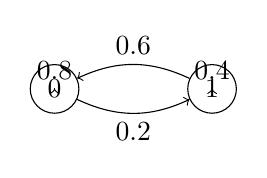
\begin{tikzpicture}[->]
\node[circle,draw] (A) at (0,0) {$0$};
\node[circle,draw] (B) at (2,0) {$1$};
\draw [->] (A) to [bend right=25] node [below,midway] {0.2} (B);
\draw [->] (B) to [bend right=25] node [above,midway] {0.6} (A);
\draw [->] (A) to [bend right=25] node [above,midway] {0.8} (A);
\draw [->] (B) to [bend right=25] node [above,midway] {0.4} (B);
\end{tikzpicture}
\caption{Graphe de transition}
\label{fig:transition}
\end{center}
\end{figure}
\end{example}

\begin{example}[Marché boursier]
A la fin de chaque jour, nous enregistre le prix de l'action de Google au marché de WallStreet:
\[
X_t =
\begin{cases}
1 & \mbox{si le prix de l'action n'a pas augmenté à la fin du jour }t; \\
0 & \mbox{si le prix de l'action a augmenté à la fin du jour }t.
\end{cases}
\]
Nous supposons de plus que la probabilité que le prix augmente demain étant donné qu'il a augmenté aujourd'hui est de 0.7, et qu'il n'a pas augmenté aujourd'hui, 0.5.
Nous avons une chaîne de Markov avec comme matrice de transition:
\[
\boldsymbol[P] =
\begin{pmatrix}
p_{00} & p_{01} \\
p_{10} & p_{11}
\end{pmatrix}
=
\begin{pmatrix}
0.7 & 0.3 \\
0.5 & 0.5
\end{pmatrix}
\]

Supposons maintenant que la probabilité que le prix de l'action augmente demain dépend non seulement de ce qui est arrivé aujourd'hui, mais également de ce qui est arrivé hier.
Le processus stochastique défini précédemment n'est alors plus une chaîne de Markov.
Nous pouvons néanmoins nous en sortir en introduisant un état pour
chaque combinaison d'états possibles sur deux jours consécutifs.
Nous définissons alors le processus stochastique suivant, où l'indice $t$ représente deux jours consécutifs:
\[
X_t =
\begin{cases}
0 & \mbox{si le prix de l'action a augmenté hier et aujourd'hui}; \\
3 & \mbox{si le prix de l'action n'a pas augmenté, ni hier, ni aujourd'hui}; \\
2 & \mbox{si le prix de l'action a augmenté hier, mais pas aujourd'hui}; \\
1 &  \mbox{si le prix de l'action a augmenté aujourd'hui, mais pas hier.}
\end{cases}
\]
Remarquons qu'il est impossible de passer de l'état 0 au temps $t$ à l'état 1 au temps $t+1$, car
$X_t = 0$, si le prix augmente hier et aujourd'hui, et $X_{t+1} = 1$, si le prix augmente demain, mais pas aujourd'hui.
La probabilité que le prix de l'action augmente demain vaut
\begin{itemize}
\item
s'il a augmenté hier et aujourd'hui: 0.9;
\item
s'il a augmenté aujourd'hui, mais pas hier: 0.6;
\item
s'il a augmenté hier, mais pas aujourd'hui: 0.5;
\item
s'il n'a pas augmenté, ni hier, ni aujourd'hui: 0.3.
\end{itemize}
La matrice de transition est
\[
\boldsymbol{P} =
\begin{pmatrix}
0.9 & 0 & 0.1 & 0 \\
0.6 & 0 & 0.4 & 0 \\
0 & 0.5 & 0 & 0.5 \\
0 & 0.3 & 0 & 0.7
\end{pmatrix}
\]
\end{example}

\begin{small}
\section{Notes}

Ce chapitre se base essentiellement sur les notes de cours de Bernard Gendron, 2007.

\end{small}
